\documentclass[11pt,a4paper]{article}
\usepackage[left=2cm,text={17cm,24cm},top=3cm]{geometry}
\usepackage[T1]{fontenc}
\usepackage[czech]{babel}
\usepackage[utf8]{inputenc}
\usepackage{url}
\usepackage{graphicx}
\usepackage{pdfpages}
\usepackage{algorithmicx}
\graphicspath{ {img/} }

\begin{document}

\begin{center}
	\LARGE{Paralelní a distribuované algoritmy -- dokumentace k projektu 1}\\
	\large{Vysoké učení technické v Brně}
	\vspace{0.5cm}

	Petr Stehlík <xstehl14@stud.fit.vutbr.cz>

	\vspace{0.2cm}

	\today

\end{center}

\section{Zadání}

Cílem projektu byla implementace algoritmu enumeration sort na lineárním poli procesorů, který byl prezentován během přednášek. Běh a kompilace programu je zprostředkován pomocí skriptu \texttt{test.sh}. Implementace využívá knihovny \textit{OpenMPI}.


\section{Rozbor a analýza algoritmu}

Enumeration sort je algoritmus pro seřazení všech prvků $x_1...x_n$ pomocí nalezení konečné pozice všech prvků v poli. Toho algoritmus docílí pomoci porovnání všech prvků $x_i$ navzájem a určením kolik ostatních prvků je menších než daný prvek $x_i$.

Enumeration sort na lineárním poli procesorů disponuje společnou sběrnicí pro všechny procesory. Tato sběrnice je schopna v každém kroku přenést jednu hodnotu a všechny procesory jsou doplněny lineárním spojením. Schéma zapojení procesorů je znázorněné na obrázku \ref{schema}.

Každý procesor obsahuje celkem 4 registry:
\begin{itemize}
    \item{C -- počet prvků menších než $x_i$},
    \item{X -- prvek $x_i$},
    \item{Y -- postupně prvky $x_1 ... x_n$},
    \item{Z -- seřazený prvek $Y_i$}.
\end{itemize}

\begin{figure}[!ht]
    \includegraphics[width=1\linewidth]{schema}
    \centering
    \caption{Schéma zapojení procesorů. Převzato z \cite{bib:schema}}
    \label{schema}
\end{figure}

Algoritmus byl modifikován tak, aby dokázal řadit i duplicitní prvky. Pořadí u duplicitních prvků algoritmus je určeno dle indexu porovnávaných identických prvků.

\subsection{Algoritmus}
\begin{enumerate}
    \item {Všechny registry C nastav na hodnotu 1}
    \item {Následující činnosti opakuj $2n$ krát, kde $1 \leq k \leq 2n$}
        \begin{itemize}
            \item{Pokud není vstup vyčerpán, vstupní prvek $x_i$ se vloží přes sběrnici do registru $X_i$ a pomocí lineárního spojení do registru $Y_1$; obsah všech registrů $Y$ se posune doprava.}
            \item{Každý procesor s neprázdnými registry $X$ a $Y$ je porovná, a je-li $X > Y$ inkrementuje svůj registr $C$}
        \end{itemize}
\end{enumerate}

\section{Implementace}

\section{Experimentální ověření časové složitosti}

\begin{figure}[!ht]
    \centering
    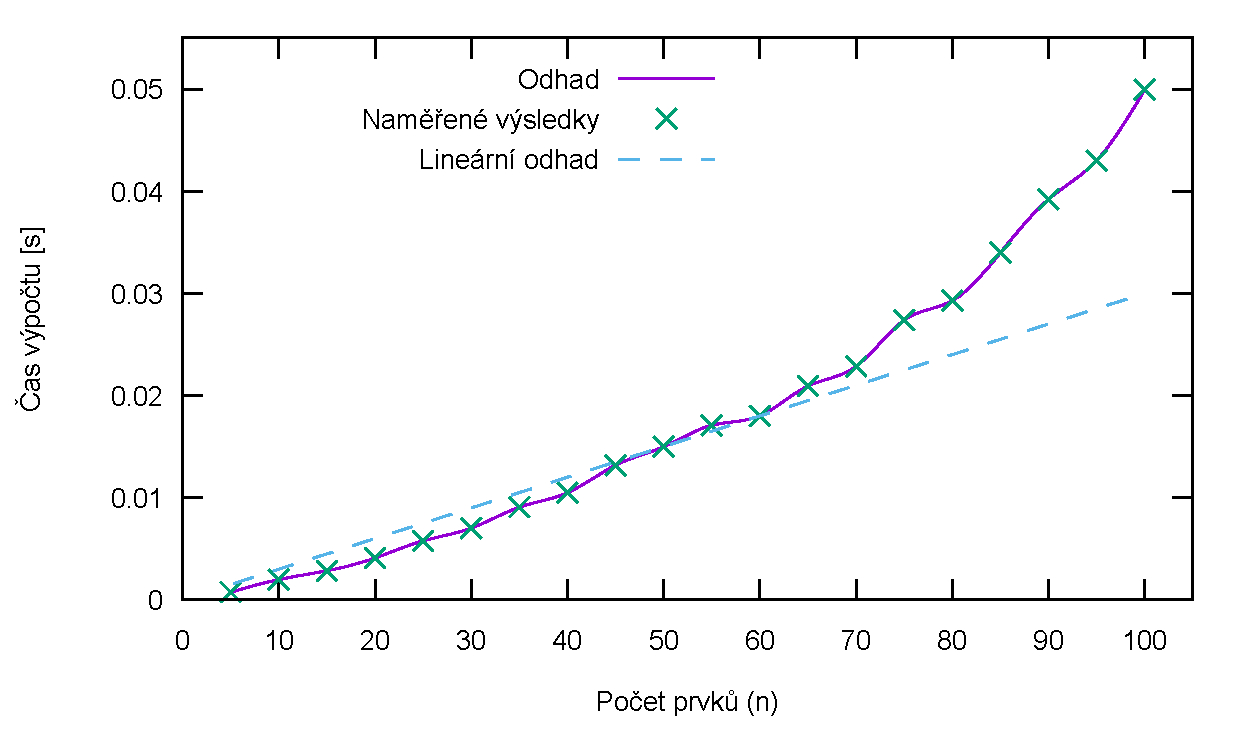
\includegraphics[width=1\textwidth]{results}
    \caption{Experimentálně naměřené výsledky}
\end{figure}

\section{Komunikační protokol}


\section{Závěr}


\bibliography{literature}

\makeatletter
\makeatother
\bibliographystyle{czechiso}

\end{document}

